\begin{figure}[h] 
\centering 
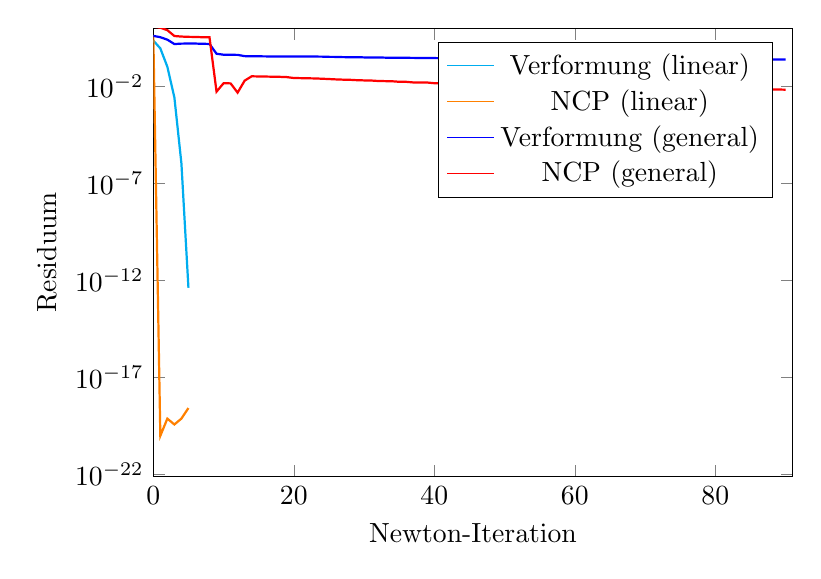
\begin{tikzpicture}[every plot/.append style={thick}] 
\begin{axis}[ 
label style={font=\normalsize}, 
xlabel={Newton-Iteration}, 
ylabel={Residuum}, 
xmin=0, xmax=91, 
ymode=log, 
ymin=0, ymax=10, 
width=0.8\textwidth, 
height=0.6\textwidth, 
legend pos=north east, 
legend style={cells={align=left}}, 
grid style=dashed, 
] 
\addplot[ 
color=cyan, 
] 
coordinates { 
(0, 2.31e+00)(1, 9.16e-01)(2, 1.03e-01)(3, 2.70e-03)(4, 1.09e-06)(5, 4.24e-13)}; 
\addlegendentry{Verformung (linear)} 
\addplot[ 
color=orange, 
] 
coordinates { 
(0, 4.39e+00)(1, 1.00e-20)(2, 7.67e-20)(3, 3.83e-20)(4, 7.67e-20)(5, 2.68e-19)}; 
\addlegendentry{NCP (linear)} 
\addplot[ 
color=blue, 
] 
coordinates { 
(0, 4.03e+00)(1, 3.45e+00)(2, 2.57e+00)(3, 1.53e+00)(4, 1.61e+00)(5, 1.62e+00)(6, 1.62e+00)(7, 1.58e+00)(8, 1.55e+00)(9, 4.84e-01)(10, 4.32e-01)(11, 4.26e-01)(12, 4.24e-01)(13, 3.65e-01)(14, 3.59e-01)(15, 3.57e-01)(16, 3.54e-01)(17, 3.52e-01)(18, 3.50e-01)(19, 3.48e-01)(20, 3.51e-01)(21, 3.50e-01)(22, 3.48e-01)(23, 3.46e-01)(24, 3.44e-01)(25, 3.35e-01)(26, 3.33e-01)(27, 3.24e-01)(28, 3.23e-01)(29, 3.22e-01)(30, 3.14e-01)(31, 3.13e-01)(32, 3.12e-01)(33, 3.05e-01)(34, 3.04e-01)(35, 3.04e-01)(36, 2.98e-01)(37, 2.97e-01)(38, 2.92e-01)(39, 2.91e-01)(40, 2.90e-01)(41, 2.85e-01)(42, 2.85e-01)(43, 2.84e-01)(44, 2.80e-01)(45, 2.80e-01)(46, 2.80e-01)(47, 2.76e-01)(48, 2.76e-01)(49, 2.75e-01)(50, 2.72e-01)(51, 2.72e-01)(52, 2.68e-01)(53, 2.68e-01)(54, 2.68e-01)(55, 2.65e-01)(56, 2.65e-01)(57, 2.65e-01)(58, 2.63e-01)(59, 2.63e-01)(60, 2.63e-01)(61, 2.60e-01)(62, 2.61e-01)(63, 2.61e-01)(64, 2.59e-01)(65, 2.59e-01)(66, 2.56e-01)(67, 2.56e-01)(68, 2.57e-01)(69, 2.54e-01)(70, 2.55e-01)(71, 2.55e-01)(72, 2.53e-01)(73, 2.53e-01)(74, 2.53e-01)(75, 2.52e-01)(76, 2.52e-01)(77, 2.52e-01)(78, 2.51e-01)(79, 2.51e-01)(80, 2.49e-01)(81, 2.49e-01)(82, 2.50e-01)(83, 2.48e-01)(84, 2.48e-01)(85, 2.46e-01)(86, 2.47e-01)(87, 2.47e-01)(88, 2.45e-01)(89, 2.46e-01)(90, 2.46e-01)}; 
\addlegendentry{Verformung (general)} 
\addplot[ 
color=red, 
] 
coordinates { 
(0, 1.21e+01)(1, 1.06e+01)(2, 7.94e+00)(3, 3.97e+00)(4, 3.72e+00)(5, 3.60e+00)(6, 3.55e+00)(7, 3.44e+00)(8, 3.40e+00)(9, 5.41e-03)(10, 1.46e-02)(11, 1.44e-02)(12, 4.80e-03)(13, 1.99e-02)(14, 3.33e-02)(15, 3.28e-02)(16, 3.23e-02)(17, 3.18e-02)(18, 3.13e-02)(19, 3.03e-02)(20, 2.72e-02)(21, 2.68e-02)(22, 2.63e-02)(23, 2.59e-02)(24, 2.50e-02)(25, 2.41e-02)(26, 2.31e-02)(27, 2.24e-02)(28, 2.20e-02)(29, 2.10e-02)(30, 2.05e-02)(31, 2.02e-02)(32, 1.91e-02)(33, 1.88e-02)(34, 1.85e-02)(35, 1.74e-02)(36, 1.73e-02)(37, 1.61e-02)(38, 1.61e-02)(39, 1.59e-02)(40, 1.47e-02)(41, 1.49e-02)(42, 1.47e-02)(43, 1.34e-02)(44, 1.38e-02)(45, 1.36e-02)(46, 1.22e-02)(47, 1.28e-02)(48, 1.26e-02)(49, 1.12e-02)(50, 1.19e-02)(51, 1.04e-02)(52, 1.13e-02)(53, 1.11e-02)(54, 9.49e-03)(55, 1.06e-02)(56, 1.04e-02)(57, 8.71e-03)(58, 9.98e-03)(59, 9.82e-03)(60, 8.01e-03)(61, 9.43e-03)(62, 9.28e-03)(63, 7.38e-03)(64, 8.96e-03)(65, 6.87e-03)(66, 8.67e-03)(67, 8.54e-03)(68, 6.36e-03)(69, 8.31e-03)(70, 8.18e-03)(71, 5.91e-03)(72, 7.99e-03)(73, 7.86e-03)(74, 5.51e-03)(75, 7.71e-03)(76, 7.59e-03)(77, 5.16e-03)(78, 7.48e-03)(79, 4.85e-03)(80, 7.39e-03)(81, 7.27e-03)(82, 4.57e-03)(83, 7.21e-03)(84, 7.10e-03)(85, 7.17e-03)(86, 7.06e-03)(87, 6.95e-03)(88, 7.04e-03)(89, 6.93e-03)(90, 6.82e-03)}; 
\addlegendentry{NCP (general)} 
\end{axis} 
\end{tikzpicture} 
\caption{Residuen des Stoffgesetzes 'Neo Hooke' mit Hinderniss 'Hut' und 2178 Freiheitsgraden für die Verschiebung.} 
\label{fiq:NeoHooke_Hut_level4} 
\end{figure} 
